\chapter{Plateforme de co-simulation et algorithme d'orchestration}\label{sec:orc}
\section*{Introduction}
Les plateformes de co-simulation nécessitent des algorithmes d'orchestration (OA) pour coordonner l'exécution des FMUs dans un scénario. L'OA définie comment les données sont échangées entre les FMUs dans le scénario et permet également d'influencer leur évolution d'état durant la co-simulation. Bien qu'il ne fasse pas partie de la norme FMI, l'OA est une caractéristique essentielle d'une plateforme de co-simulation. Des études ont démontré qu'il a un impact considérable sur l'exactitude des résultats de la co-simulation\cite{b7}.


Malheureusement, il n'y a pas de solution open source pour la co-simulation qui combine flexibilité, facilité d'usage et performances. Ce manque oblige ceux qui veulent personnaliser leur processus ou expérimenter avec de nouveaux algorithmes à construire leur propre système depuis le début ou reprendre un énorme travail de choix et compréhension des plateformes existantes (en prenant en compte les problèmes de licence). Ceci est particulièrement chronophage pour les grands projets, car il faut coder manuellement toutes les interactions entre les unités de simulation, prolongeant ainsi la phase préparatoire avant même de commencer à optimiser la co-simulation.

Dans ce chapitre, on va présenter une comparaison des différentes plateformes open source, où on va spécifier les points forts et faibles de chacune et argumenter le choix de notre plateforme de base (OMSimulator \cite{b14}). D'autre part, on présente le processus de développement d'un orchestrateur basé sur la méthode d'Aitken-Schwarz \cite{b27,b28}.

\section{Plateformes de co-simulation}
Le standard FMI joue un rôle essentiel dans les plateformes de co-simulation, en facilitant l'intégration et l'interopérabilité des modèles entre différents outils. Des plateformes notables comme Dymola, OpenModelica, Simulink, Maestro2 et Open Simulation Platform (OSP) utilisent largement la norme FMI pour améliorer leurs capacités de simulation. Dymola \cite{17} permet un échange de modèles et une co-simulation efficaces grâce à l'interface FMI, et prend en charge divers domaines. OpenModelica a développé OMSimulator \cite{b14}, qui peut servir comme une plateforme de co-simulation indépendante à base du standard FMI. Simulink \cite{b17}, de MATLAB, prend en charge le standard FMI à la fois en tant qu'importateur et exportateur, s'intégrant ainsi de manière transparente dans les flux de travail multi-outils. Maestro2 \cite{b13}, offre de solides fonctions de co-simulation à l'aide de FMI, visant à simplifier l'intégration de systèmes multidisciplinaires complexes. DACCOSIM NG \cite{b15}, la dernière version de la plateforme de co-simulation Daccosim, offre plusieurs fonctionnalités notamment la distribution de la co-simulation. PyFMI \cite{b16} est un package Python qui offre une interface pour travailler avec des modèles basés sur le standard FMI.
Enfin, OSP \cite{18} est une plateforme de co-simulation axée sur l'industrie maritime.

\subsection{Limites et choix}
La création d'une plateforme de co-simulation à partir de zéro est souvent inefficace et coûteuse en ressources, étant donnée la complexité de l'intégration et de la maintenance requise. Opter pour une base existante permet non seulement de réduire significativement le temps et les efforts de développement, mais aussi d'assurer une compatibilité et une robustesse initiale. La sélection d'une plateforme appropriée s'oriente selon des critères —tels que la personnalisation, les performances, SSP\footnote{Le standard SSP (System Structure and Parameterization) est conçu pour améliorer l'interopérabilité entre différents outils de simulation en permettant une description structurée des systèmes et de leurs paramètres.}, et la documentation— qui sont détaillés dans la figure \ref{fig:21}. Cette approche stratégique favorise une réalisation plus efficace des objectifs de l'étude, concentrant les efforts sur la personnalisation plutôt que sur la construction initiale.

\begin{table}[hbt!]
    \centering
    \caption{Comparaison basée sur divers critères}
    \begin{tabular}{@{}lccccc@{}} % Notice the change here to accommodate two more columns
    \toprule
    Critère & OMSimulator & Maestro2 & OSP & pyFMI & Daccosim NG \\ % Added pyFMI and Daccosim NG
    \midrule
    Personnalisation & \twochecks & \threechecks & \onecheck & \twochecks & \onecheck \\ % Example data
    Performances & \threechecks & \threechecks & \onecheck & \twochecks & \twochecks \\ % Example data
    Documentation & \threechecks & \onecheck & \nocheck & \twochecks & \onecheck \\ % Example data
    Facilité d'utilisation & \threechecks & \onecheck & \twochecks & \threechecks & \twochecks \\ % Example data
    Support de SSP  & \threechecks & \twochecks & \twochecks & \twochecks & \onecheck \\ % Example data
    Modularité & \twochecks & \threechecks & \onecheck & \nocheck & \twochecks \\ % Example data
    Distribution & \nocheck & \nocheck & \nocheck & \twochecks & \threechecks \\ % Example data
    Langage  & C++ & Java & C++ & Python & C++ \\ % Adjusted to include programming languages
    \bottomrule
    \end{tabular}
    \label{fig:21}
\end{table}

J'ai opté pour OMSimulator pour plusieurs raisons convaincantes. Tout d'abord, il bénéficie d'une documentation riche et accessible, ce qui facilite grandement l'apprentissage et l'utilisation de l'outil. Sa structure et sa conception soignées garantissent également une expérience utilisateur fluide et aisée. De plus, OMSimulator est un outil déjà bien développé, offrant une base solide pour tout projet de co-simulation. Un autre point fort est l'activité continue de son équipe de développement sur GitHub, ce qui témoigne de leur engagement à améliorer constamment l'outil et à soutenir sa communauté d'utilisateurs. Cette combinaison de facteurs fait d'OMSimulator le choix idéal pour ce projet.

\subsection{OMSimulator}

OMSimulator \cite{b14} est développé en tant que bibliothèque de simulation autonome en open source, dotée d'une interface utilisateur complète en C. Son intégration dans l'éditeur graphique OpenModelica OMEdit illustre l'utilisation de l'interface C-API pour créer une expérience utilisateur graphique et intuitive. En outre, OMSimulator propose une interface en ligne de commande (CLI), des interfaces de script pour Python et Lua, permettant son intégration dans divers outils tiers et applications spécialisées, tels que des simulateurs de vol.

Dans OMS, les modèles composites sont structurés sous forme d'un arbre hiérarchique composé de blocs de construction spécifiques. Le nœud racine de cet arbre peut être un système TLM, un système faiblement couplé (système WC) ou un système fortement couplé (système SC), chacun se distinguant par la manière dont les connexions sont gérées : 
\begin{itemize}
    \item Les systèmes \textbf{TLM} contiennent des connexions TLM, qui peuvent être considérées comme des connexions retardées motivées par la physique.
    \item Les systèmes faiblement couplés \textbf{Weakly-Coupled} sont utilisés pour la co-simulation. Toutes les unités de simulation fonctionnent de manière indépendante et sont synchronisées par un algorithme maître à certains moments de la communication.
    \item Les systèmes fortement couplés \textbf{Strongly-Coupled} sont utilisés pour regrouper les FMUs-ME dans une unité de co-simulation. Ils partagent un solveur commun et utilisent un schéma de communication continu. 
\end{itemize}
On a étudié la documentation générée à travers Doxygen\footnote{\url{https://www.doxygen.nl/}} et le source code fournit\footnote{\url{https://github.com/OpenModelica/OMSimulator}} afin de créer une documentation plus ciblée qui servira de guide pour les futures modifications par l'équipe RTSIM. Cette documentation spécifique est présentée dans l'annexe \ref{app:documentation}.  Il est important de noter que notre étude se concentre particulièrement sur l'approche des systèmes faiblement couplés (WC) et que tous les FMUs utilisés pour les démonstrations dans cette recherche sont des FMUs-CS.

\subsection{Interface d'utilisation OMS}

Dans notre contexte, on se sert de la version lignes des commandes, ainsi que l'interface python pour la rédaction des scénarios de co-simulation. 

Dans la configuration d'OMSimulatorPython, le fichier `capi.py` joue un rôle essentiel puisqu'il utilise `ctypes`, une bibliothèque Python pour appeler des fonctions C depuis Python. Cela permet aux scripts Python d'accéder directement et d'utiliser les fonctionnalités de simulation sous-jacentes fournies par OMSimulator. En utilisant `ctypes` pour établir des liaisons avec des fonctions C, `capi.py` convertit efficacement ces fonctions en fonctions que l'on peut invoquer en Python. Autour de ce fichier central, d'autres modules Python tels que `Model.py`, `System.py`, et `Scope.py` s'appuient sur ces liaisons pour offrir une API plus abstraite, permettant aux utilisateurs de gérer les  scénarios de co-simulation plus facilement. Cette architecture non seulement simplifie l'intégration de tâches de simulation complexes dans les scripts Python, mais maintient également les avantages de performance de l'implémentation C native, comblant ainsi le fossé entre la facilité de scriptage de haut niveau et la puissance computationnelle de bas niveau.

Dans la figure \ref{tab:A2}, on présente un script Python pour lancer une co-simulation d'un amplificateur différentiel divisé en deux FMUs comme présenté dans la figure suivante :

\begin{figure}[hbt!]
    \centering
    \begin{minipage}[b]{0.45\textwidth}
        \includegraphics[width=\textwidth]{leftfmu.png}
    \end{minipage}
    \begin{minipage}[b]{0.45\textwidth}
      \includegraphics[width=\textwidth]{rightfmu.png}
  \end{minipage}
  \caption{Modèles des FMUs utilisés dans la co-simulation de l'amplificateur différentiel}
  \label{fig:21}
  \end{figure}

  \section{Génération des FMUs}
  Transformer un modèle ou un ensemble d'équations en un FMU , qui compile essentiellement ces éléments en un ensemble de code C et de bibliothèques, présente un ensemble unique de défis et d'opportunités. Cette transformation implique l'encapsulation du comportement dynamique du modèle dans une unité compilée autonome qui interagit avec divers environnements de simulation via le standard FMI. Cependant, la compilation multi-plateforme représente un problème notable. Assurer le fonctionnement sans faille d'un FMU sur différents systèmes d'exploitation (Windows, Linux, MacOS) peut être complexe en raison des différences entre les compilateurs, les bibliothèques et les architectures systèmes.
  
  On présente quelques outils de génération des FMUs testés dans cette étude : 
  \begin{itemize}
    \item \textbf{SIMULINK} :  On utilise le Simulink Coder en combinaison avec le FMI Kit pour générer des FMUs à partir des modèles Simulink. Cette méthode permet d'exporter les modèles sous forme de FMUs, supportant la co-simulation ou l'échange de modèles. Le processus inclut la configuration du modèle Simulink pour l'exportation, la sélection des réglages appropriés du solveur, puis l'utilisation de la fonction d'exportation du FMI Kit pour finaliser l'exportation.
    \item \textbf{OpenModelica} : OpenModelica offre un support intégré pour l'exportation de modèles sous forme de FMUs. On charge simplement le modèle dans OpenModelica et on utilise la commande exportToFMU(). Cette commande permet de spécifier différentes options, telles que la compatibilité de version (FMI 1.0 ou 2.0), et le choix entre l'exportation pour la co-simulation ou l'échange de modèles. On peut également utiliser le drapeau supplémentaire "-d=fmuExperimental". Ce drapeau permet d'activer des fonctionnalités expérimentales spécifiques qui ne sont pas encore standard dans la version stable de OpenModelica tel que : fmi2GetSpecificDerivatives, canGetSetFMUState, canSerializeFMUstate.
    \item \textbf{Source Code FMU (pythonfmu)} : Ces dernières années, plusieurs cadres logiciels open-source ont été développés pour l'exportation des FMUs à partir du code source. CPPFMU, développé par SINTEF Ocean dans le cadre du projet ViProMa, propose une interface C++ de haut niveau avec des fonctionnalités telles que les exceptions et la gestion automatique de la mémoire pour écrire du code maîtres/esclaves conforme à FMI. Cependant, il ne prend pas en charge la génération du fichier 'modelDescription.xml' ni le conditionnement des FMUs. FMUSDK, fourni par QTronic, est un SDK basé sur C permettant l'utilisation des FMUs pour l'échange de modèles et la co-simulation, et qui supporte jusqu'à la version 2.0 de FMI, mais il manque également la génération automatique du modelDescription.xml. JavaFMI, développé par l'institut SIANI et financé par l'EIFER, et FMI4j, développé en Kotlin et sous licence MIT, prennent tous deux en charge l'importation et l'exportation de FMUs sur la JVM, FMI4j utilise CPPFMU pour la mise en œuvre des fonctions FMI et se concentre sur la performance grâce à l'intégration JNI. JavaFMI emploie une approche plus impérative utilisant le passage de messages, tandis que FMI4j utilise un style déclaratif avec des annotations, conduisant à des différences dans la performance et l'interaction utilisateur dans la définition du modèle.
    \begin{table}[hbt!]
        \centering
        \begin{tabular}{|c|c|c|c|}
          \hline
          \textbf{Tool} & \textbf{Target language} & \textbf{Target platform} & \textbf{FMI version} \\ \hline
          JavaFMI & JVM & Win, Linux & 2.0 \\ \hline
          FMI4j & JVM & Win, Linux & 2.0 \\ \hline
          CPPFMU & C++ & Win, Linux  & 1.0 \& 2.0 \\ \hline
          FMUSDK & C & Win, Linux, OSX  & 1.0 \& 2.0 \\ \hline
          Pythonfmu & python & Win, Linux & 1.0 \& 2.0 \\
          \hline
        \end{tabular}
        \caption{Comparaison des différents outils d'export des FMUs}
      \end{table}

      PythonFMU \footnote{\url{https://github.com/NTNU-IHB/PythonFMU}} \cite{26} est une plateforme logicielle sous licence MIT qui facilite l'empaquetage de code Python "3.x" en FMUs de co-simulation. Développé en collaboration entre NTNU et Safran Tech, il est accessible via pip ou conda. Bien qu'il fonctionne immédiatement sur les systèmes Windows et Linux 64 bits, PythonFMU requiert une distribution Python compatible déjà installée sur le système cible, ainsi que toute bibliothèque tierce nécessaire. On présente dans \ref{tab:A3}, notre script python pour créer un FMU correspondant à une source de courant.
    \item \textbf{uniFmu} \footnote{\url{https://github.com/INTO-CPS-Association/unifmu/tree/}} \cite{27}: Universal Functional Mock-up Unit est un outil qui permet l'implémentation des FMUs dans n'importe quel langage de programmation. Ce framework fournit des binaires pré-compilés pour Windows, Linux et macOS, évitant ainsi les complications liées à la cross-compilation et à la configuration de chaînes d'outils complexes. Il intègre également un mécanisme d'extension facile à utiliser, permettant la prise en charge de divers langages de programmation. De plus, une interface en ligne de commande est disponible pour générer rapidement des FMUs à l'aide d'une seule commande.
  \end{itemize}

  \section{Orchestration de la co-simulation}
  L'algorithme orchestrateur est chargé de gérer l'échange de données et la synchronisation entre ses composants, assurant ainsi que la simulation globale respecte les contraintes temporelles et les exigences de précision préétablies. Il prend en charge des tâches telles que la gestion des pas de temps, le contrôle des erreurs et la séquence d'exécution des différentes unités de simulation. En orchestrant la manière et le moment où ces FMUs échangent des données, l'algorithme maître vise à assurer que les simulations restent cohérentes et pertinentes.
\subsection{Orchestrateurs d'OMS}

Comme mentionné dans \ref{sec:WC}, on s'intéresse à la classe SystemWC.cpp. On présente dans cette section les deux algorithmes orchestrateurs d'OMS.
\begin{table}[h]
    \centering
    \begin{adjustbox}{width=\textwidth}
    
    \begin{tabular}{|c|c|c|}
    \hline
    \textbf{Solveur} & \textbf{Type} & \textbf{Description} \\ \hline
    oms\_solver\_wc\_ma & wc-system & Algorithme maître par défaut à pas fixe \\ \hline
    oms\_solver\_wc\_mav & wc-system & Algorithme maître à pas adaptatif \\ \hline
    oms\_solver\_wc\_mav2 & wc-system & Algorithme maître à pas adaptatif (double pas) \\
    \hline
    \end{tabular}
\end{adjustbox}
    \caption{Description des orchestrateurs utilisés dans les systèmes wc}
    \end{table}

    On note d'abord des points en commun entre ces différents orchestrateurs: 
    \begin{itemize}
        \item Méthode \textbf{stepUntil} : Responsable de l'avancement du temps des différents FMUs présents dans le scénario. 
        \item Méthode \textbf{getInputAndOutput} : Cette méthode traite les connexions entre les composants au sein d'un graphe dirigé pour extraire et gérer les valeurs d'entrée et de sortie pour les FMUs capables de gérer leur propre état. Elle parcourt les connexions triées, en excluant les boucles algébriques, et remplit les vecteurs avec les valeurs des signaux réels des composants FMU connectés.
        \item Méthode \textbf{SolveAlgLoop} : Cette méthode offre à l'utilisateur le choix entre deux solveurs pour résoudre les boucles algébriques, en fonction de la complexité du problème. KINSOL de SUNDIALS est idéal pour les systèmes d'équations non linéaires complexes grâce à ses méthodes robustes comme celles de Newton, adaptées aux modèles de grande envergure nécessitant des calculs précis de Jacobien. En revanche, FixedPointIteration (Algorithme de Tarjan) est plus adapté pour les systèmes moins complexes, utilisant une itération de point fixe qui permet une résolution rapide et efficace pour des problèmes d'ingénierie standard.
    \end{itemize}

Dans \ref{tab:A4}, on décrit l'algorithme qui illustre le fonctionnement de l'algorithme maître utilisant une taille de pas adaptative. Le principe repose sur la gestion de l'erreur, définie comme la différence entre les interfaces de deux états successifs, où le système est régulé en fonction de la magnitude de l'erreur. Cette dernière est indicative du dynamisme du système. On note trois points faibles de cet algorithme : 
\begin{itemize}
    \item \textbf{Contrôle de la Taille de Pas} : Si les tailles de pas maximum et minimum sont mal ajustées, cela pourrait empêcher la convergence de l'algorithme ou causer de l'instabilité par des pas trop grands.
    \item \textbf{Gestion des Erreurs} : La méthode calcule l'erreur et utilise un facteur de sécurité pour décider des rollbacks. Une mauvaise calibration de ces seuils peut entraîner des rollbacks inutiles ou insuffisants, affectant l'efficacité et la précision de la simulation.
    \item \textbf{Stabilité numérique et convergence}: L'algorithme ajuste dynamiquement les tailles de pas en fonction de la réponse du système, ce qui présente un risque d'instabilité numérique si les ajustements de pas ne sont pas en accord avec les propriétés numériques du système. Cela pourrait entraîner des solutions qui ne convergent pas ou un comportement divergent, particulièrement dans les systèmes sensibles ou très dynamiques.
\end{itemize}

Dans \ref{tab:A6}, on décrit l'algorithme utilisé par oms\_solver\_wc\_ma, qui implémente une méthode de pas fixe pour la simulation. Cet algorithme intègre également la sauvegarde des états des composants pour permettre des rollbacks en cas d'erreurs durant les étapes de simulation. Deux aspects critiques de cet algorithme sont notés :
\begin{itemize}
    \item \textbf{Adaptabilité aux Modèles Non Linéaires et Complexes}: Les simulations qui impliquent des modèles non linéaires ou ayant des comportements complexes posent des défis particuliers pour les méthodes à pas fixe. 
    \item \textbf{Critères de Convergence}: Pour garantir que l'algorithme aboutisse à une solution correcte et stable, il est important d'établir des critères de convergence bien définis et bien personnalisé. Dans le cas d'une méthode à pas fixe, où le seul degré de liberté réside dans la modification des dérivées des signaux d'entrée, cette approche peut s'avérer limitée face à la dynamique de certains systèmes.
\end{itemize}
Cela met en lumière l'importance d'adopter une méthode qui marie l'adaptabilité du pas de communication, l'optimisation des critères de convergence, et une gestion d'erreur solide, tout en maintenant la complexité des calculs à un niveau minimal.

\section{Orchestrateur Aitken-Schwarz}

Dans les sections précédentes, nous avons abordé plusieurs problèmes et défis liés à la co-simulation, incluant l'instabilité causée par le pas de communication et les mécanismes d'estimation et de contrôle d'erreurs. Ces difficultés sont largement reconnues et étudiées dans la littérature scientifique. Dans \cite{29}, une méthode itérative est proposée, qui assure la cohérence des interfaces tout en éliminant les discontinuités à chaque macro-étape. Cette méthode a été comparée à d'autres approches bien établies, telles que la co-simulation non itérative type Jacobi, la co-simulation itérative avec conservation de l'ordre zéro \cite{b12}, et un algorithme non itératif amélioré pour le lissage des variables \cite{30}. 

Dans notre travail, nous considérons un algorithme de couplage en point fixe basé sur la technique de décomposition du domaine de Schwarz dans lequel nous avons utilisé un Schwarz additif (ASM) \cite{b27}. Ces méthodes itératives peuvent être convergentes ou divergentes en fonction du partitionnement du domaine et des conditions aux limites. En outre, nous avons utilisé la propriété de convergence ou de divergence purement linéaire (c'est-à-dire que l'opérateur d'erreur de la méthode ne dépend pas du nombre d'itérations) pour accélérer la méthode itérative vers la vraie solution avec la technique d'accélération de la convergence d'Aitken, même avec une méthode divergente \cite{b28}.

Il est important de noter que, dans notre contexte, l'accélération est spécifiquement appliquée à la résolution de l'interface. De plus, ces méthodes sont non intrusives pour les FMUs, ce qui les rend particulièrement adaptées à la co-simulation de systèmes de type boîte noire (FMU-CS).



\subsection{Implémentation de la méthode Aitken-Schwarz}

On note $z(t_n)$ le vecteur contenant les différents variables de l’interface du modèle au pas de communication $t_n$, où $z(t_n) \in \mathbb{R}^N$. Le vecteur $z(t_{n+1})$ l'interface après un pas de communication (c'est-à-dire après un appel de la fonction \textbf{stepUntil} $\mathcal{S}$).
\begin{equation}
    z(t_{n+1}) = \mathcal{S} (z(t_n))
\end{equation}

Le principe de cette méthode consiste à réaliser, au cours d'un unique pas de communication, plusieurs itérations (c'est-à-dire de multiples pas de simulation sans progression temporelle), jusqu'à ce que le critère de convergence soit atteint ou qu'une limite maximale d'itérations soit dépassée.

\begin{equation}
    Z^{k+1}= \mathcal{S} (Z^{k})
\end{equation}
où k est l'indice d'itérations de Schwarz. En outre, comme montré dans \cite{b28}: 
\begin{equation}
    Z^{k+1}-Z^0 = \mathbb{P} (Z^k-Z^0)
\end{equation}
on peut extraire de l'équation (2.3) la forme généralisé de l’accélération d'aitken:
\begin{equation}
    Z^{\infty} = (Id_N - \mathbb{P} )^{-1} (Z^{1}-\mathbb{P} Z^0)
\end{equation}
En définissant l'erreur entre les valeurs à l'interface pour les itérations (k+1) et (k) de la manière suivante : $e^k = (Z^{k+1}-Z^k)$, il est possible de calculer algébriquement l'opérateur $\mathbb{P}\in\mathbb{R}^{N\cdot N}$ à partir de l'équation (2.3) après $N+1$ itérations. Cette démarche est réalisable si la matrice $[e^N,\dots, e^1]$ est inversible, et s'effectue de la manière suivante : 
\begin{equation}
    \mathbb{P} = [e^{N+1},\dots, e^2]\cdot[e^N,\cdots, e^1]^{-1}
\end{equation}
Cet opérateur d'erreur doit uniquement être calculé lors de la première étape. Toutefois, si la topologie évolue ou en présence de non-linéarités, il sera nécessaire de recalculer l'opérateur.\cite{b28}

La méthode a été implémenté dabs un méta-modèle de co-simulation et testé avec un circuit RL. Le code correspondant est présenté dans \ref{tab:A7}.
\subsection{Implémentation dans OMSimulator}

L'algorithme qui décrit l'intégration de la méthode Aitken-Schwarz dans OMS est présenté dans la figure ci-dessous :
\begin{figure}[hbt!]
    \label{fig:AS} 
    \centering
    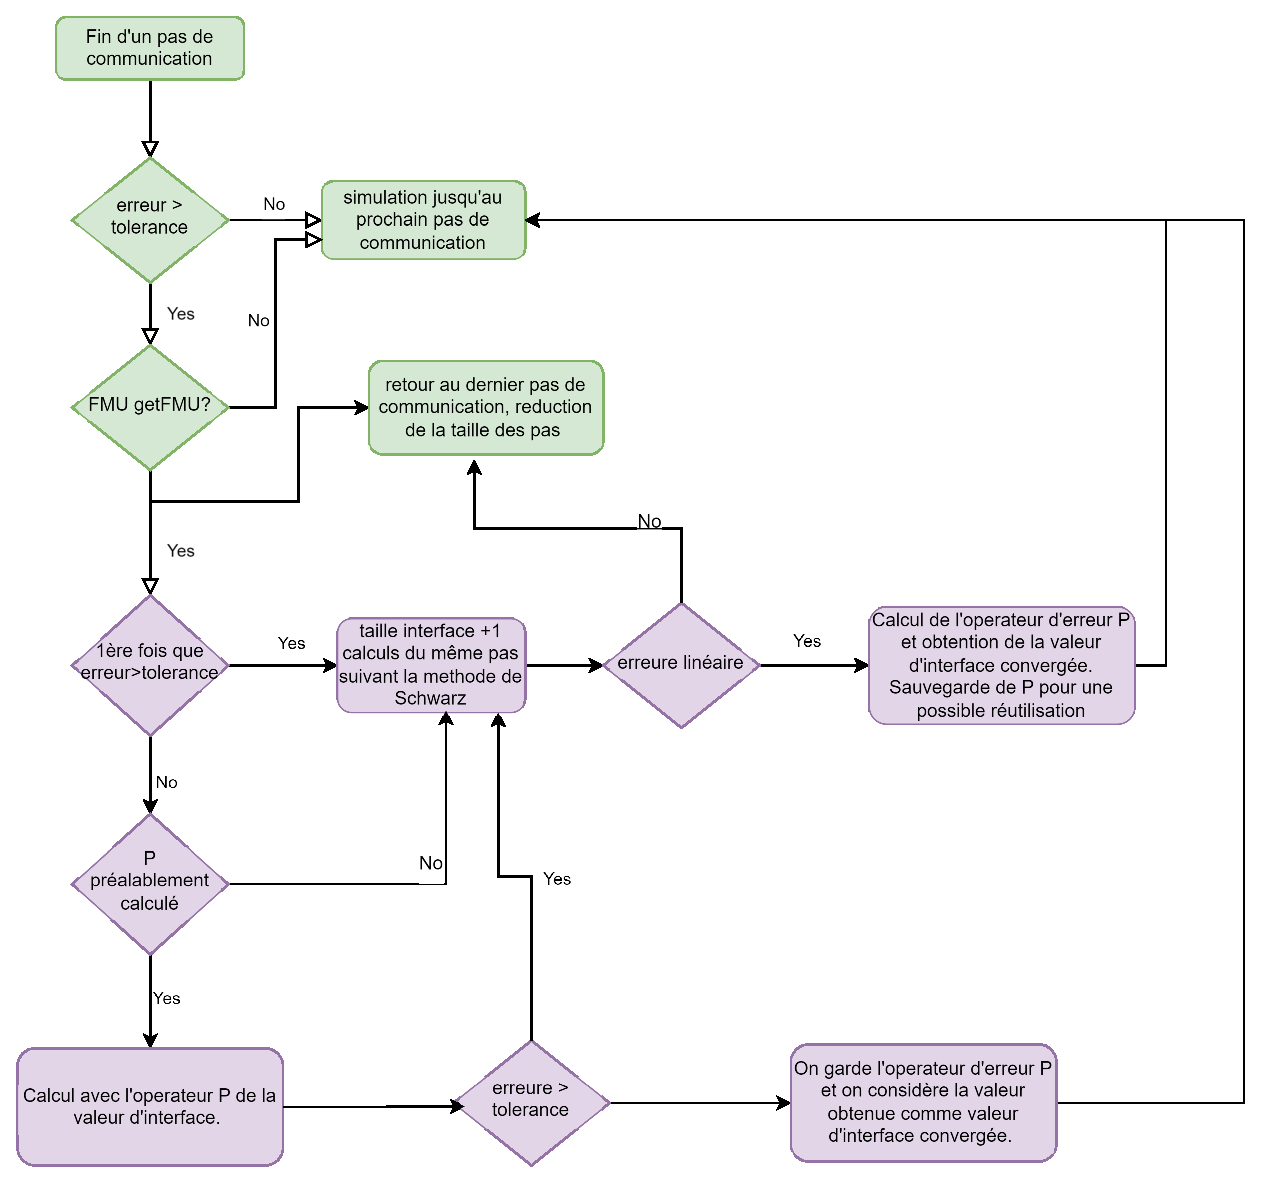
\includegraphics[width = 0.9\textwidth]{ajoutAitkenOPS.drawio.eps}
    \caption{Intégration de la méthode Aitken-Schwarz dans l'orchestrateur}
\end{figure}

L'algorithme repose sur le principe du rollback et requiert donc des FMUs compatibles avec cette fonctionnalité.
\subsection{Tests et résultats}

Pour générer des scénarios de co-simulation, on a découpé des modèles OpenModelica, avant de les exporter sous forme de FMUs. On effectue dans cette section, des tests et comparaison entre trois algorithmes orchestrateurs : 
-  oms\_solver\_wc\_ma (Rollback et modification de dérivée) - oms\_solver\_wc\_AS (Rollback et Aitken-Schwarz) - Orchestrateur simple avec tolérance relative.
 
\begin{figure}[hbt!]
    \centering
    \begin{minipage}[b]{0.45\textwidth}
        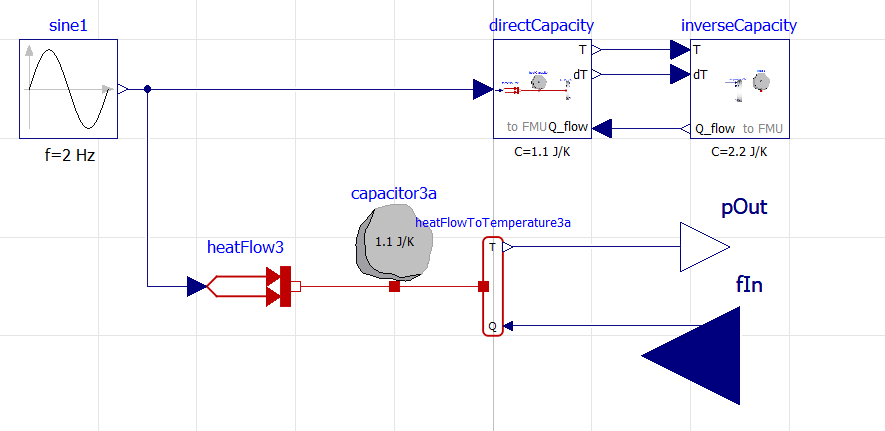
\includegraphics[width=\textwidth]{GenerationfmuL.png}
    \end{minipage}
    \begin{minipage}[b]{0.45\textwidth}
      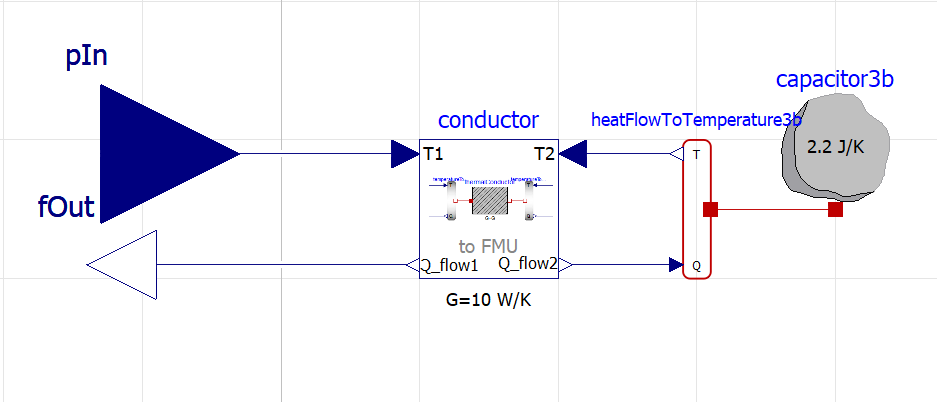
\includegraphics[width=\textwidth]{GenerationfmuR.png}
  \end{minipage}
  \caption{Modèles des FMUs utilisés dans la co-simulation de l'amplificateur différentiel}
  \label{fig:23}
  \end{figure}
Ce modèle est utilisé pour effectuer une co-simulation d'un système thermique avec une entrée sinusoïdale influençant des propriétés thermiques telles que la capacité et la conductance. On a découpé le modèle pour créer un point d'échange (pOut (Température T) et fIn (Flux de chaleur Q)). On présente dans la figure \ref{fig:24} une comparaison entre la simulation monolithique du modèle et sa co-simulation avec l'orchestrateur à pas fixe 'ma' d'OMS.

\begin{figure}[hbt!]
    \centering
    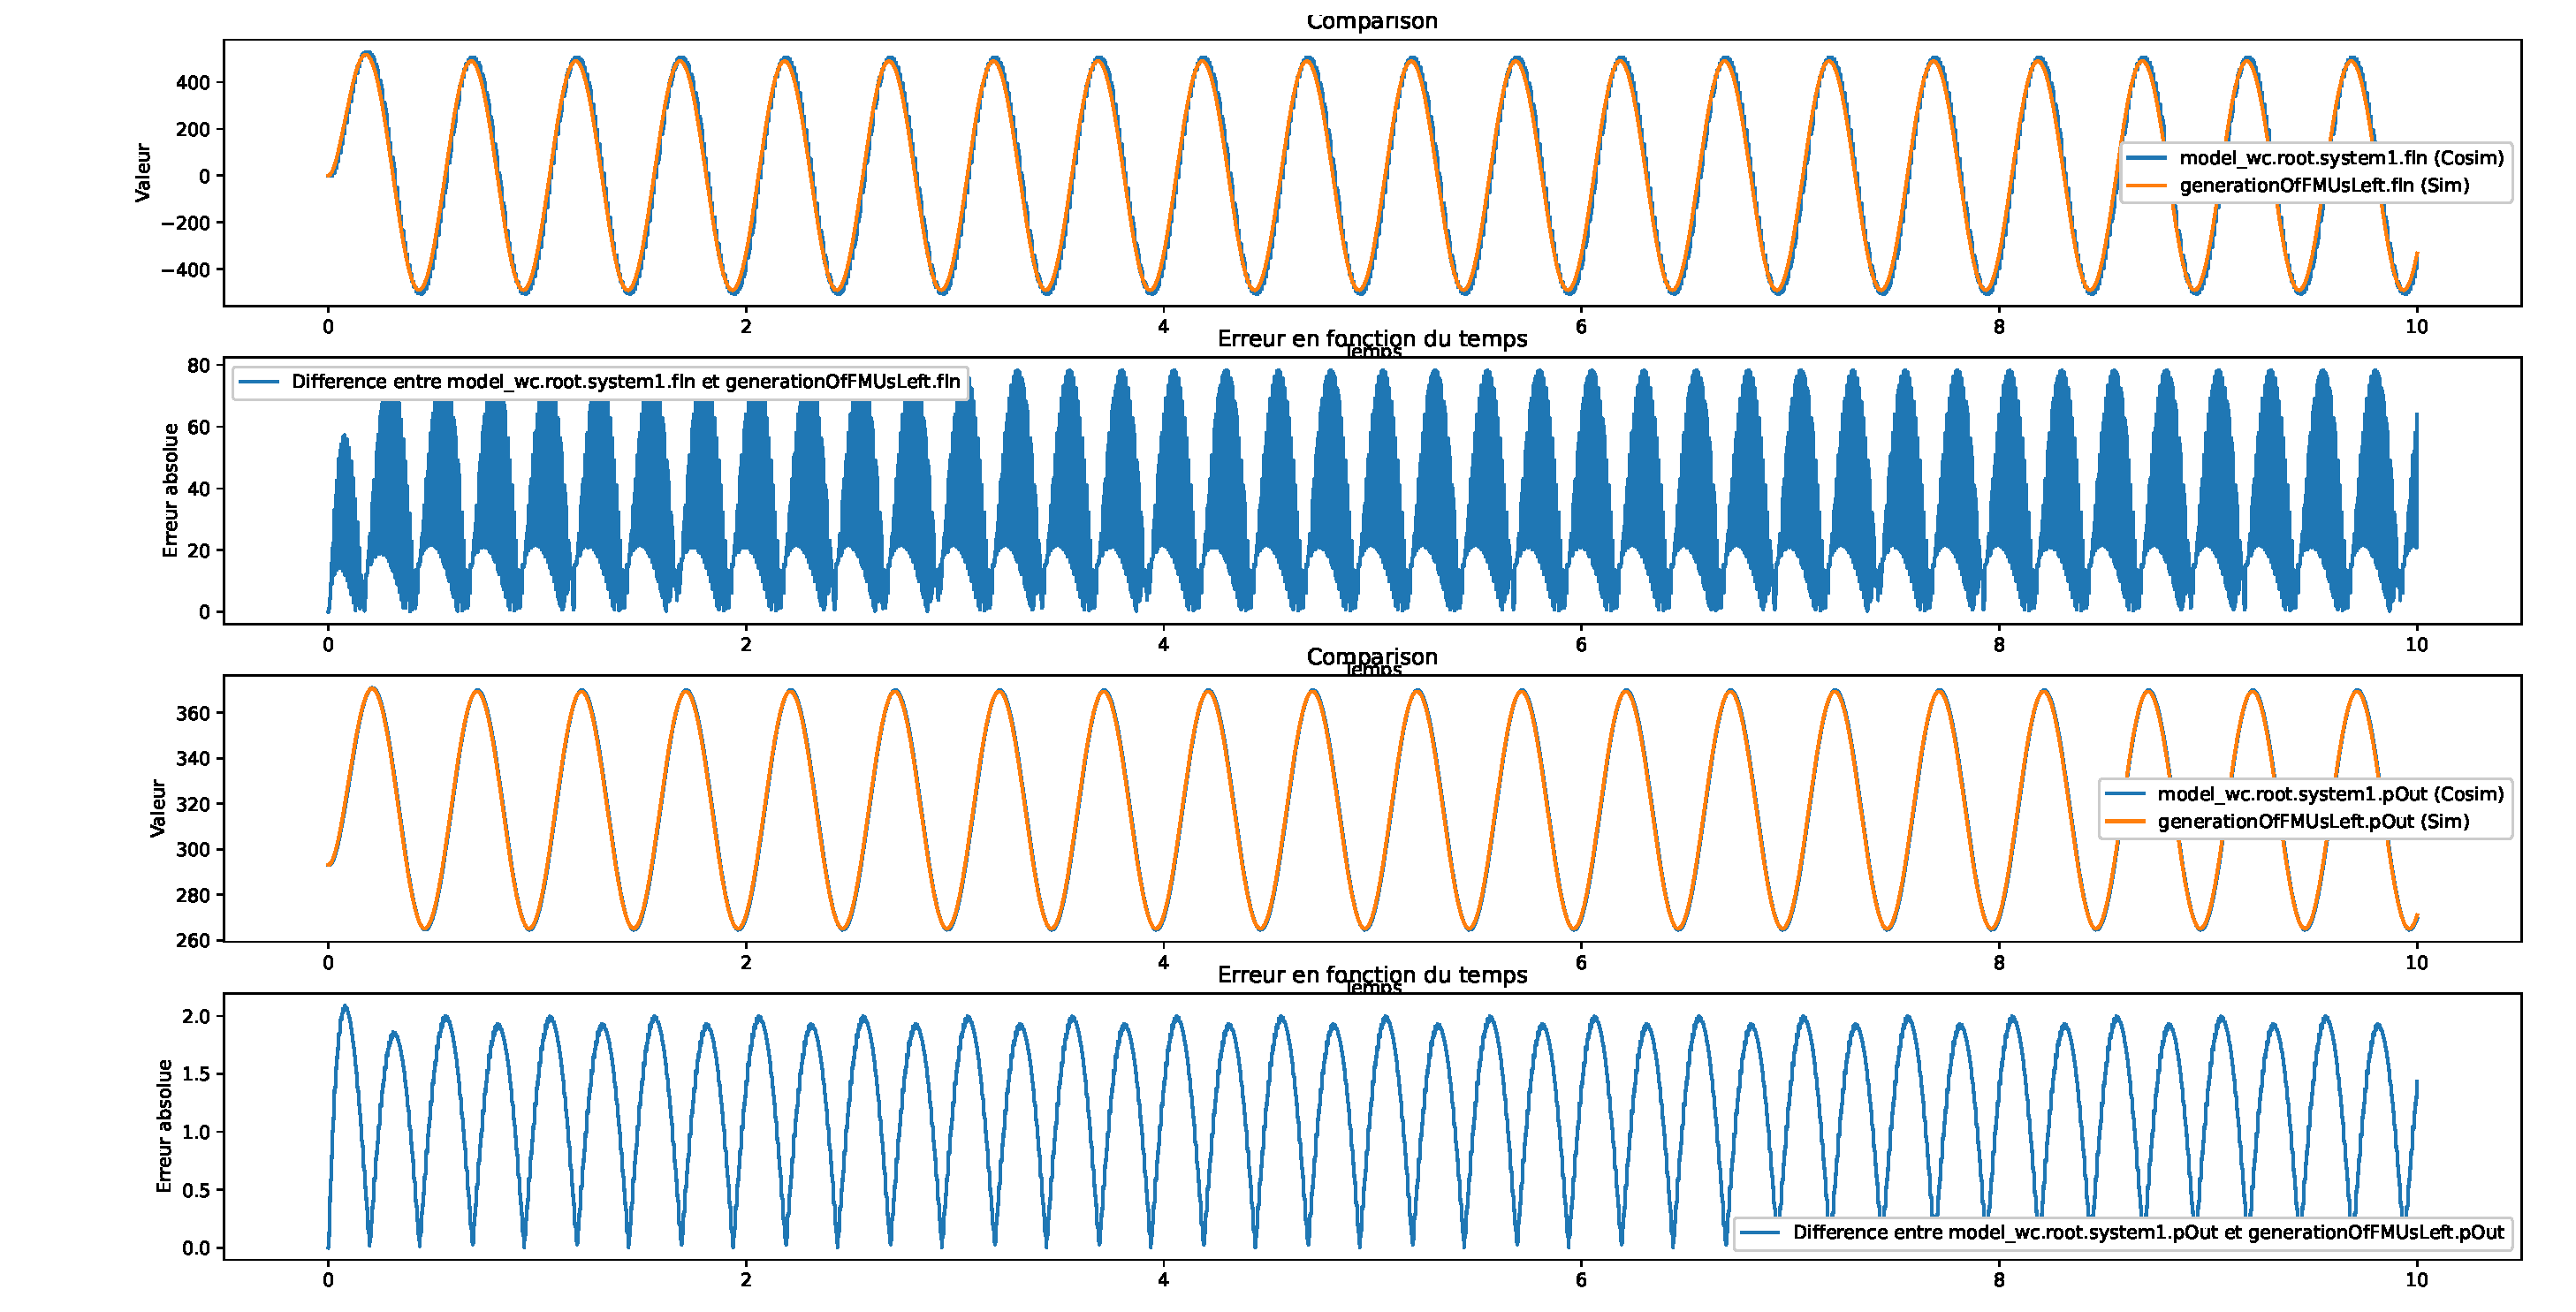
\includegraphics[width =\textwidth]{generationFMUOMS.eps}
    \caption{Comparaison de l'orchestrateur d'OMS avec une simulation monolithique du modèle \ref{fig:23}}
    \label{fig:24}
\end{figure}

Dans la figure \ref{fig:25}, nous présentons une comparaison similaire en utilisant notre orchestrateur Aitken-Schwarz. Les deux figures incluent également l'erreur absolue entre l'algorithme souhaité et la simulation monolithique du modèle. Les paramètres préfixés par "generationOffFMUs" proviennent de la simulation monolithique, tandis que ceux commençant par "model\_wc.root.systemX" sont issus de la co-simulation.
\newpage
\begin{figure}[hbt!]
    \centering
    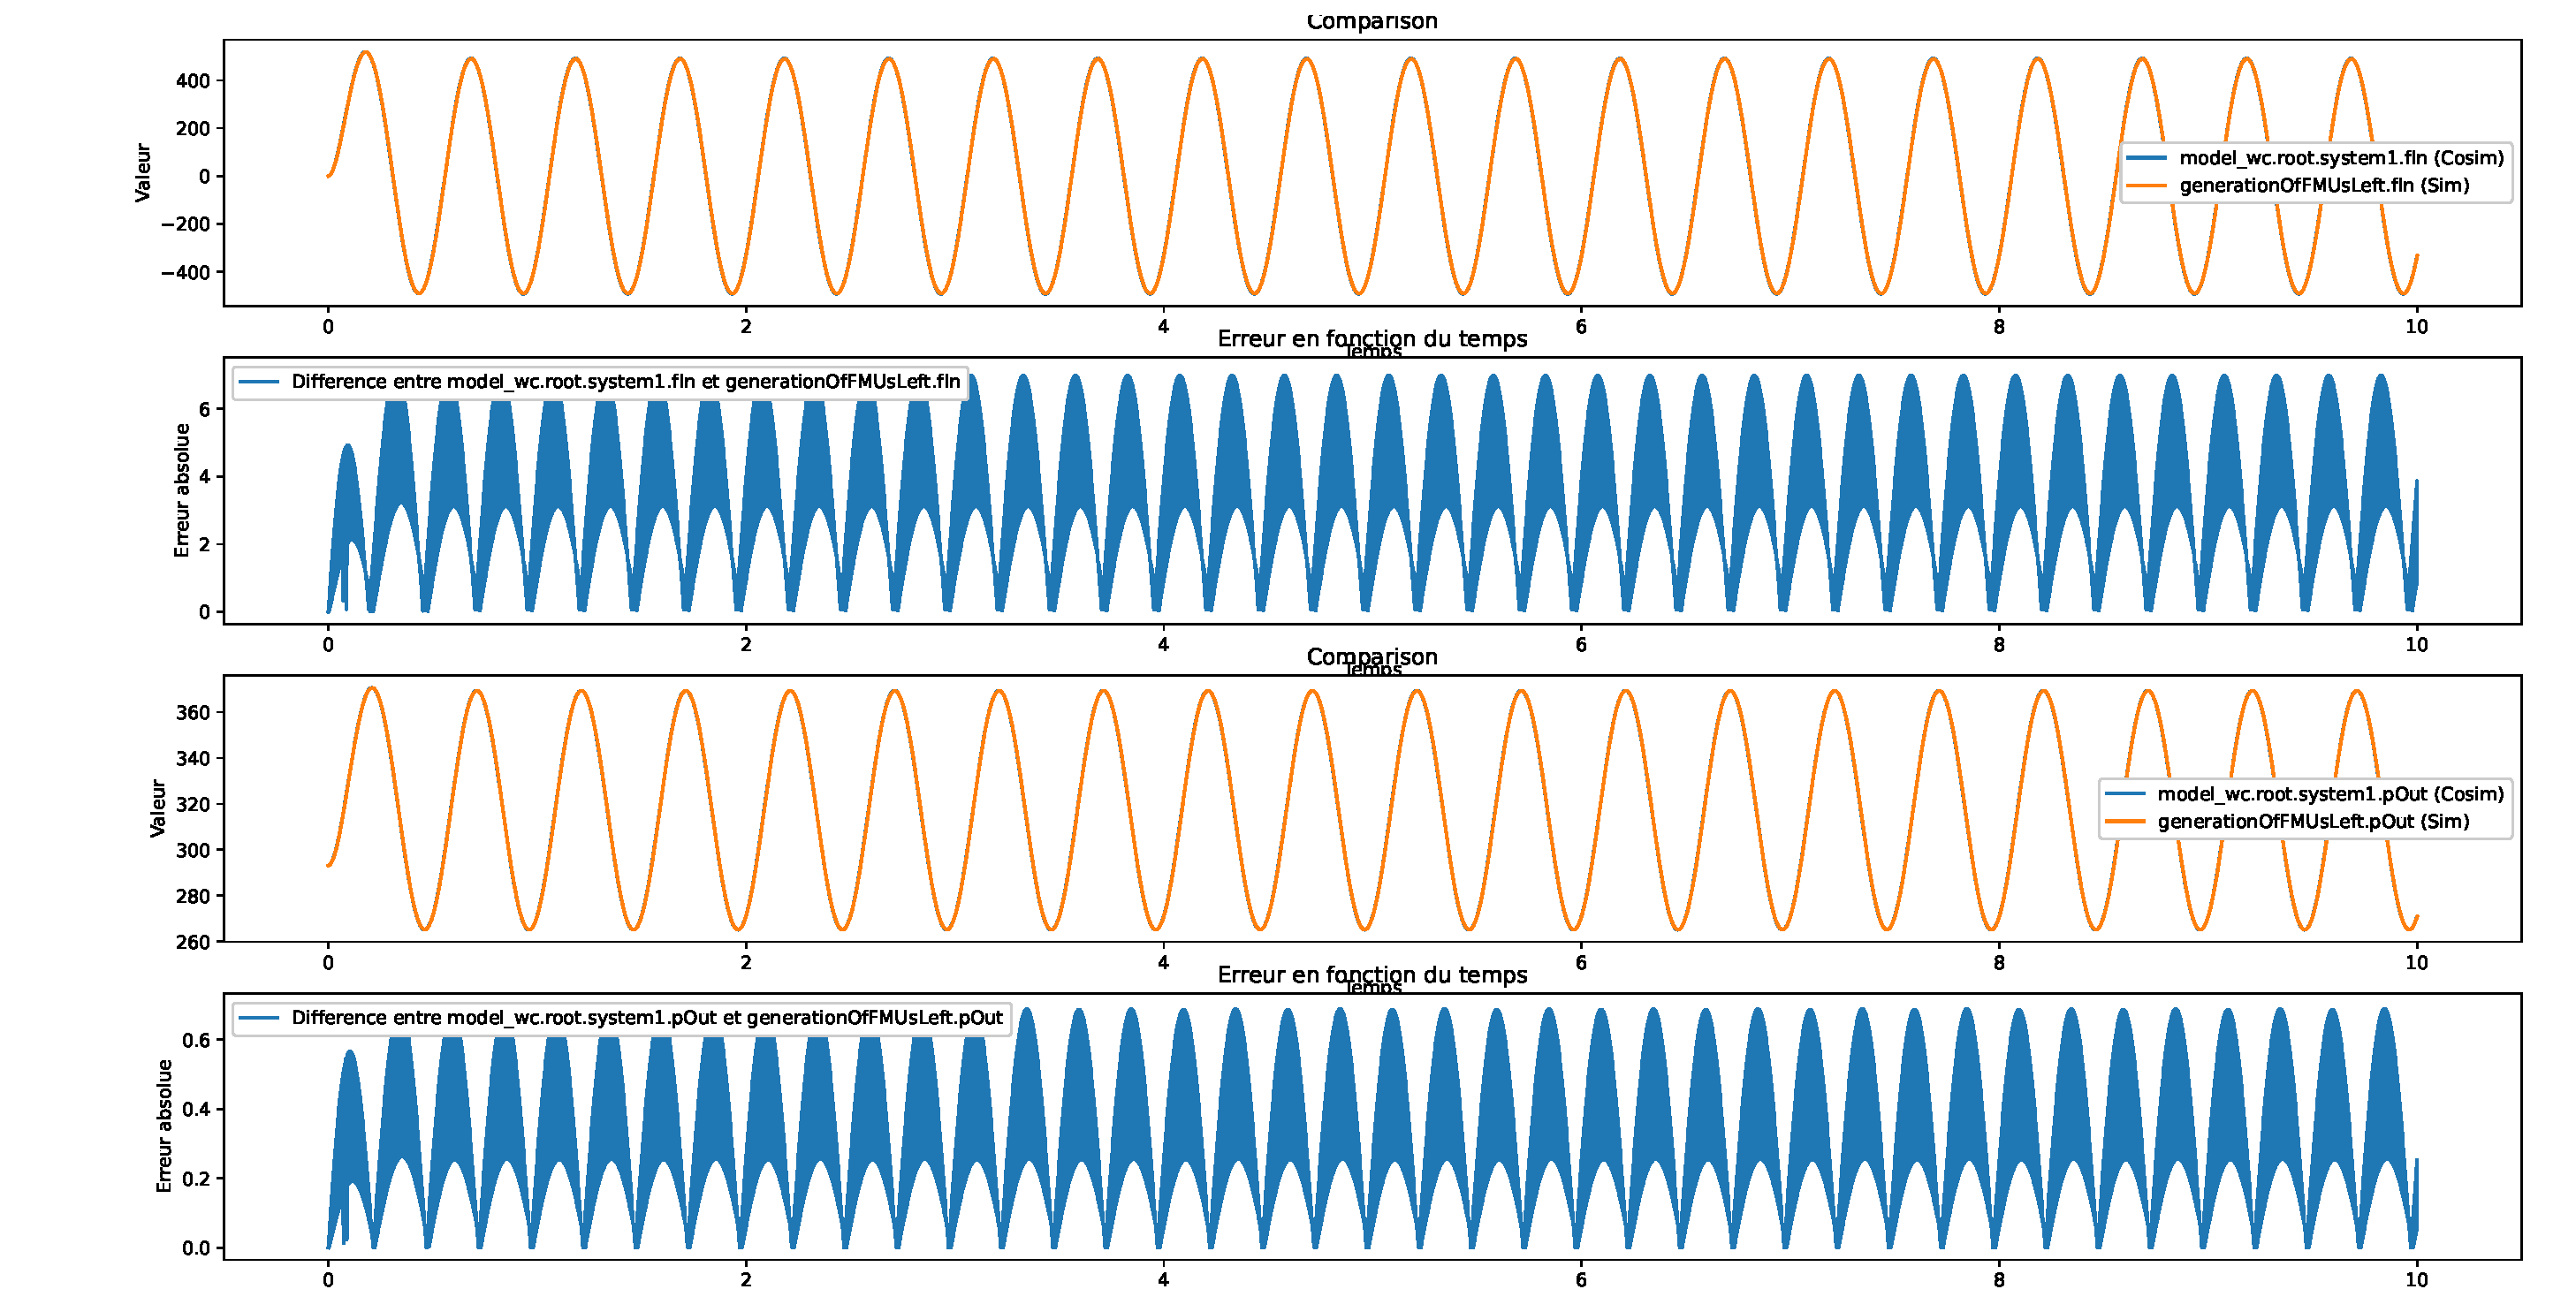
\includegraphics[width =\textwidth]{generationFMUSchwarz.eps}
    \caption{Comparaison de l'orchestrateur Aitken-Schwarz avec une simulation monolithique du modèle \ref{fig:23}}
    \label{fig:25}
\end{figure}
\begin{figure}[hbt!]
    \centering
    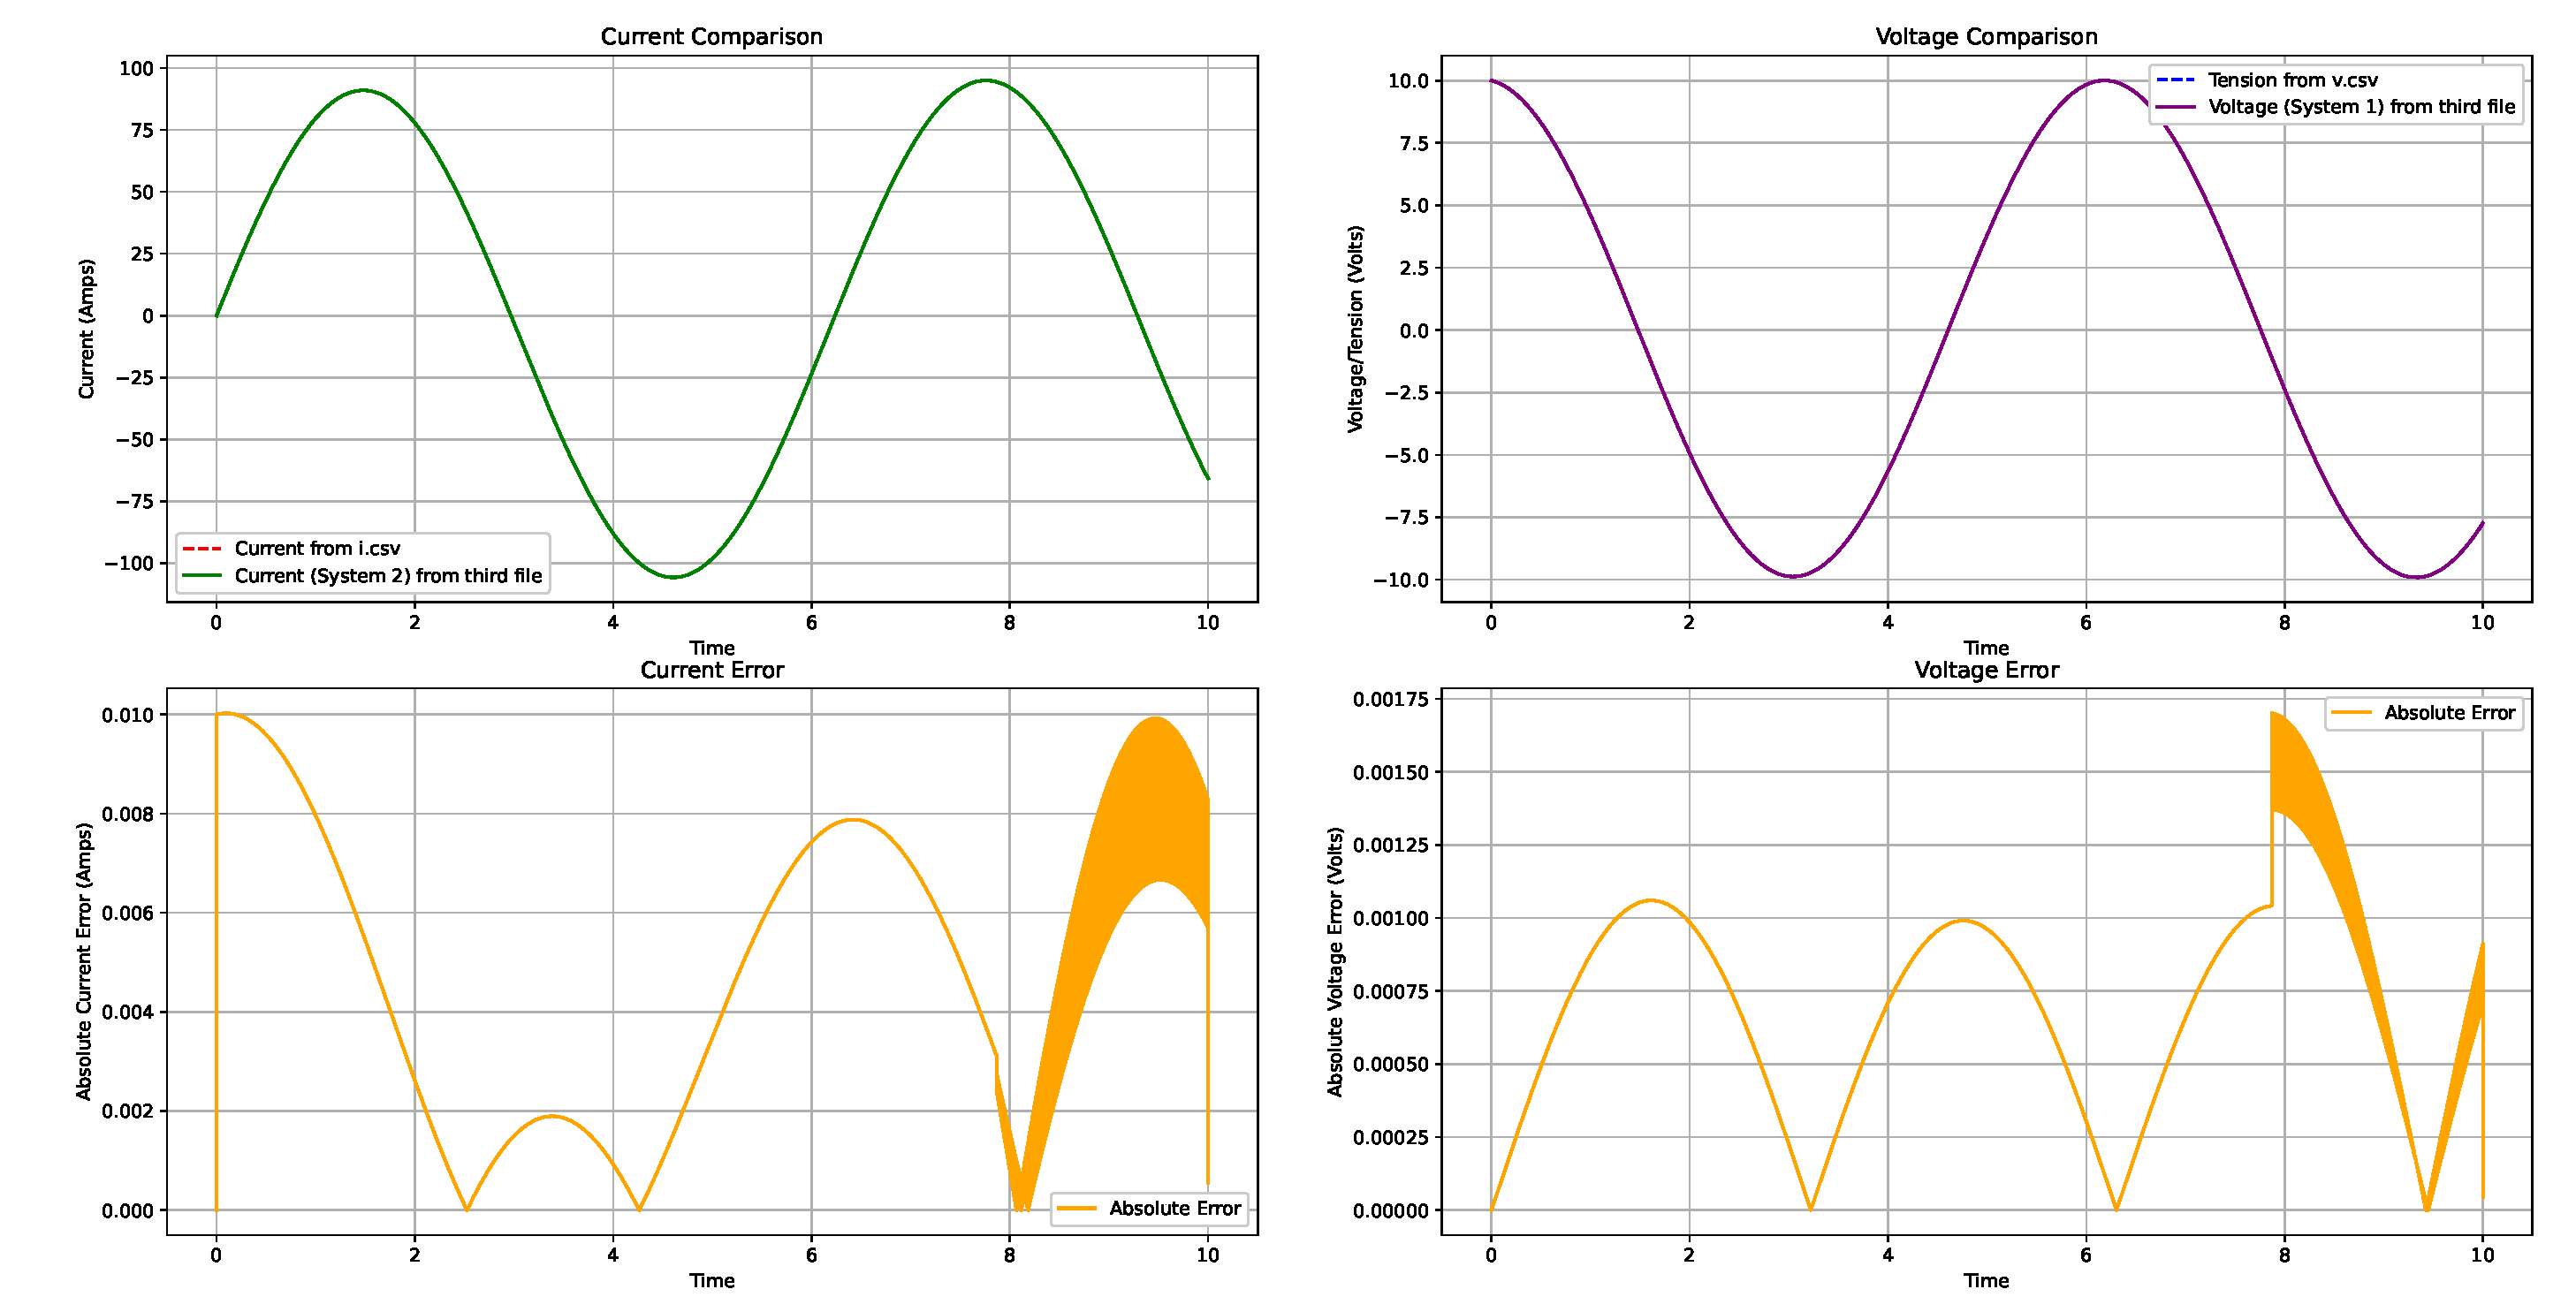
\includegraphics[width =\textwidth]{RLschwarz.eps}
    \caption{Comparaison de l'orchestrateur Aitken-Schwarz avec une simulation monolithique du circuit RL}
    \label{fig:26}
\end{figure}

On a aussi testé la méthode sur un circuit RL : 
\begin{equation}
    V_0 \cos(t) = RI + L \frac{dI}{dt}
\end{equation}
Où le circuit est divisé en deux FMUs : l'un comprend la source de tension et la résistance, et l'autre contient une bobine. Les résultats de cette configuration sont exposés dans la figure \ref{fig:26}. Les variables portant le suffixe (System) proviennent de la co-simulation. L'erreur absolue entre les résultats de la co-simulation et ceux de la simulation monolithique est également présentée.

\begin{figure}[hbt!]
    \centering
    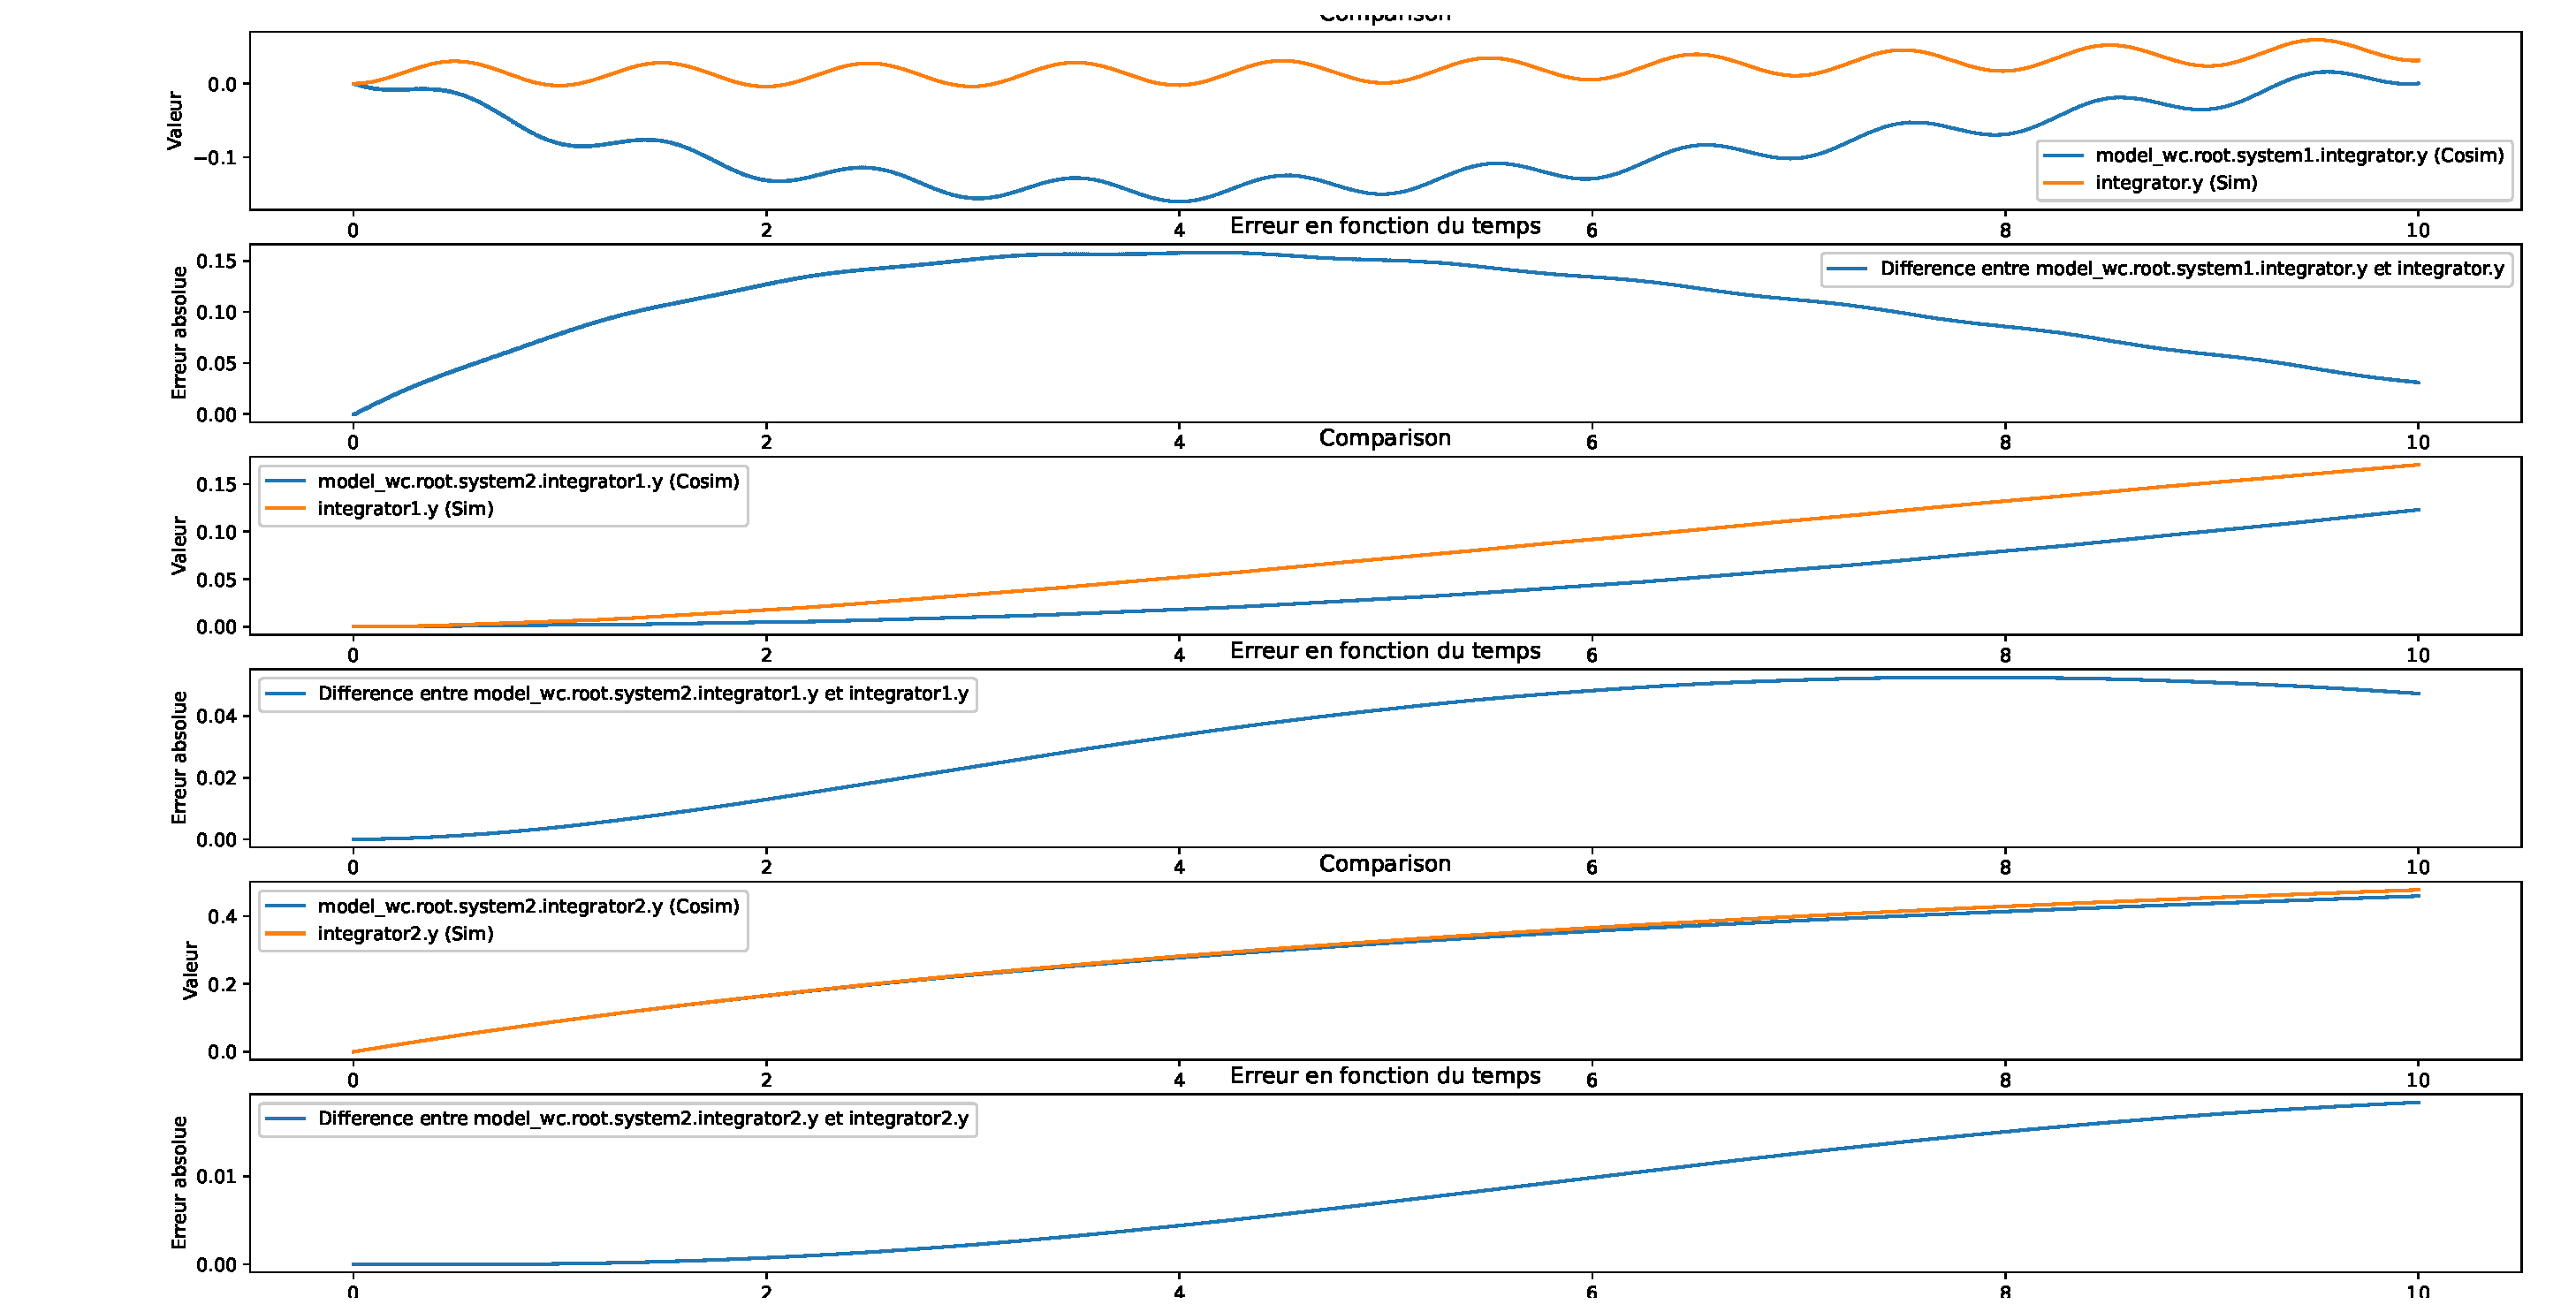
\includegraphics[width =\textwidth]{chainevolOMS.eps}
    \caption{Comparaison de l'orchestrateur Aitken-Schwarz avec une simulation monolithique du modèle \ref{fig:29}}
    \label{fig:27}
\end{figure}

\begin{figure}[hbt!]
    \centering
    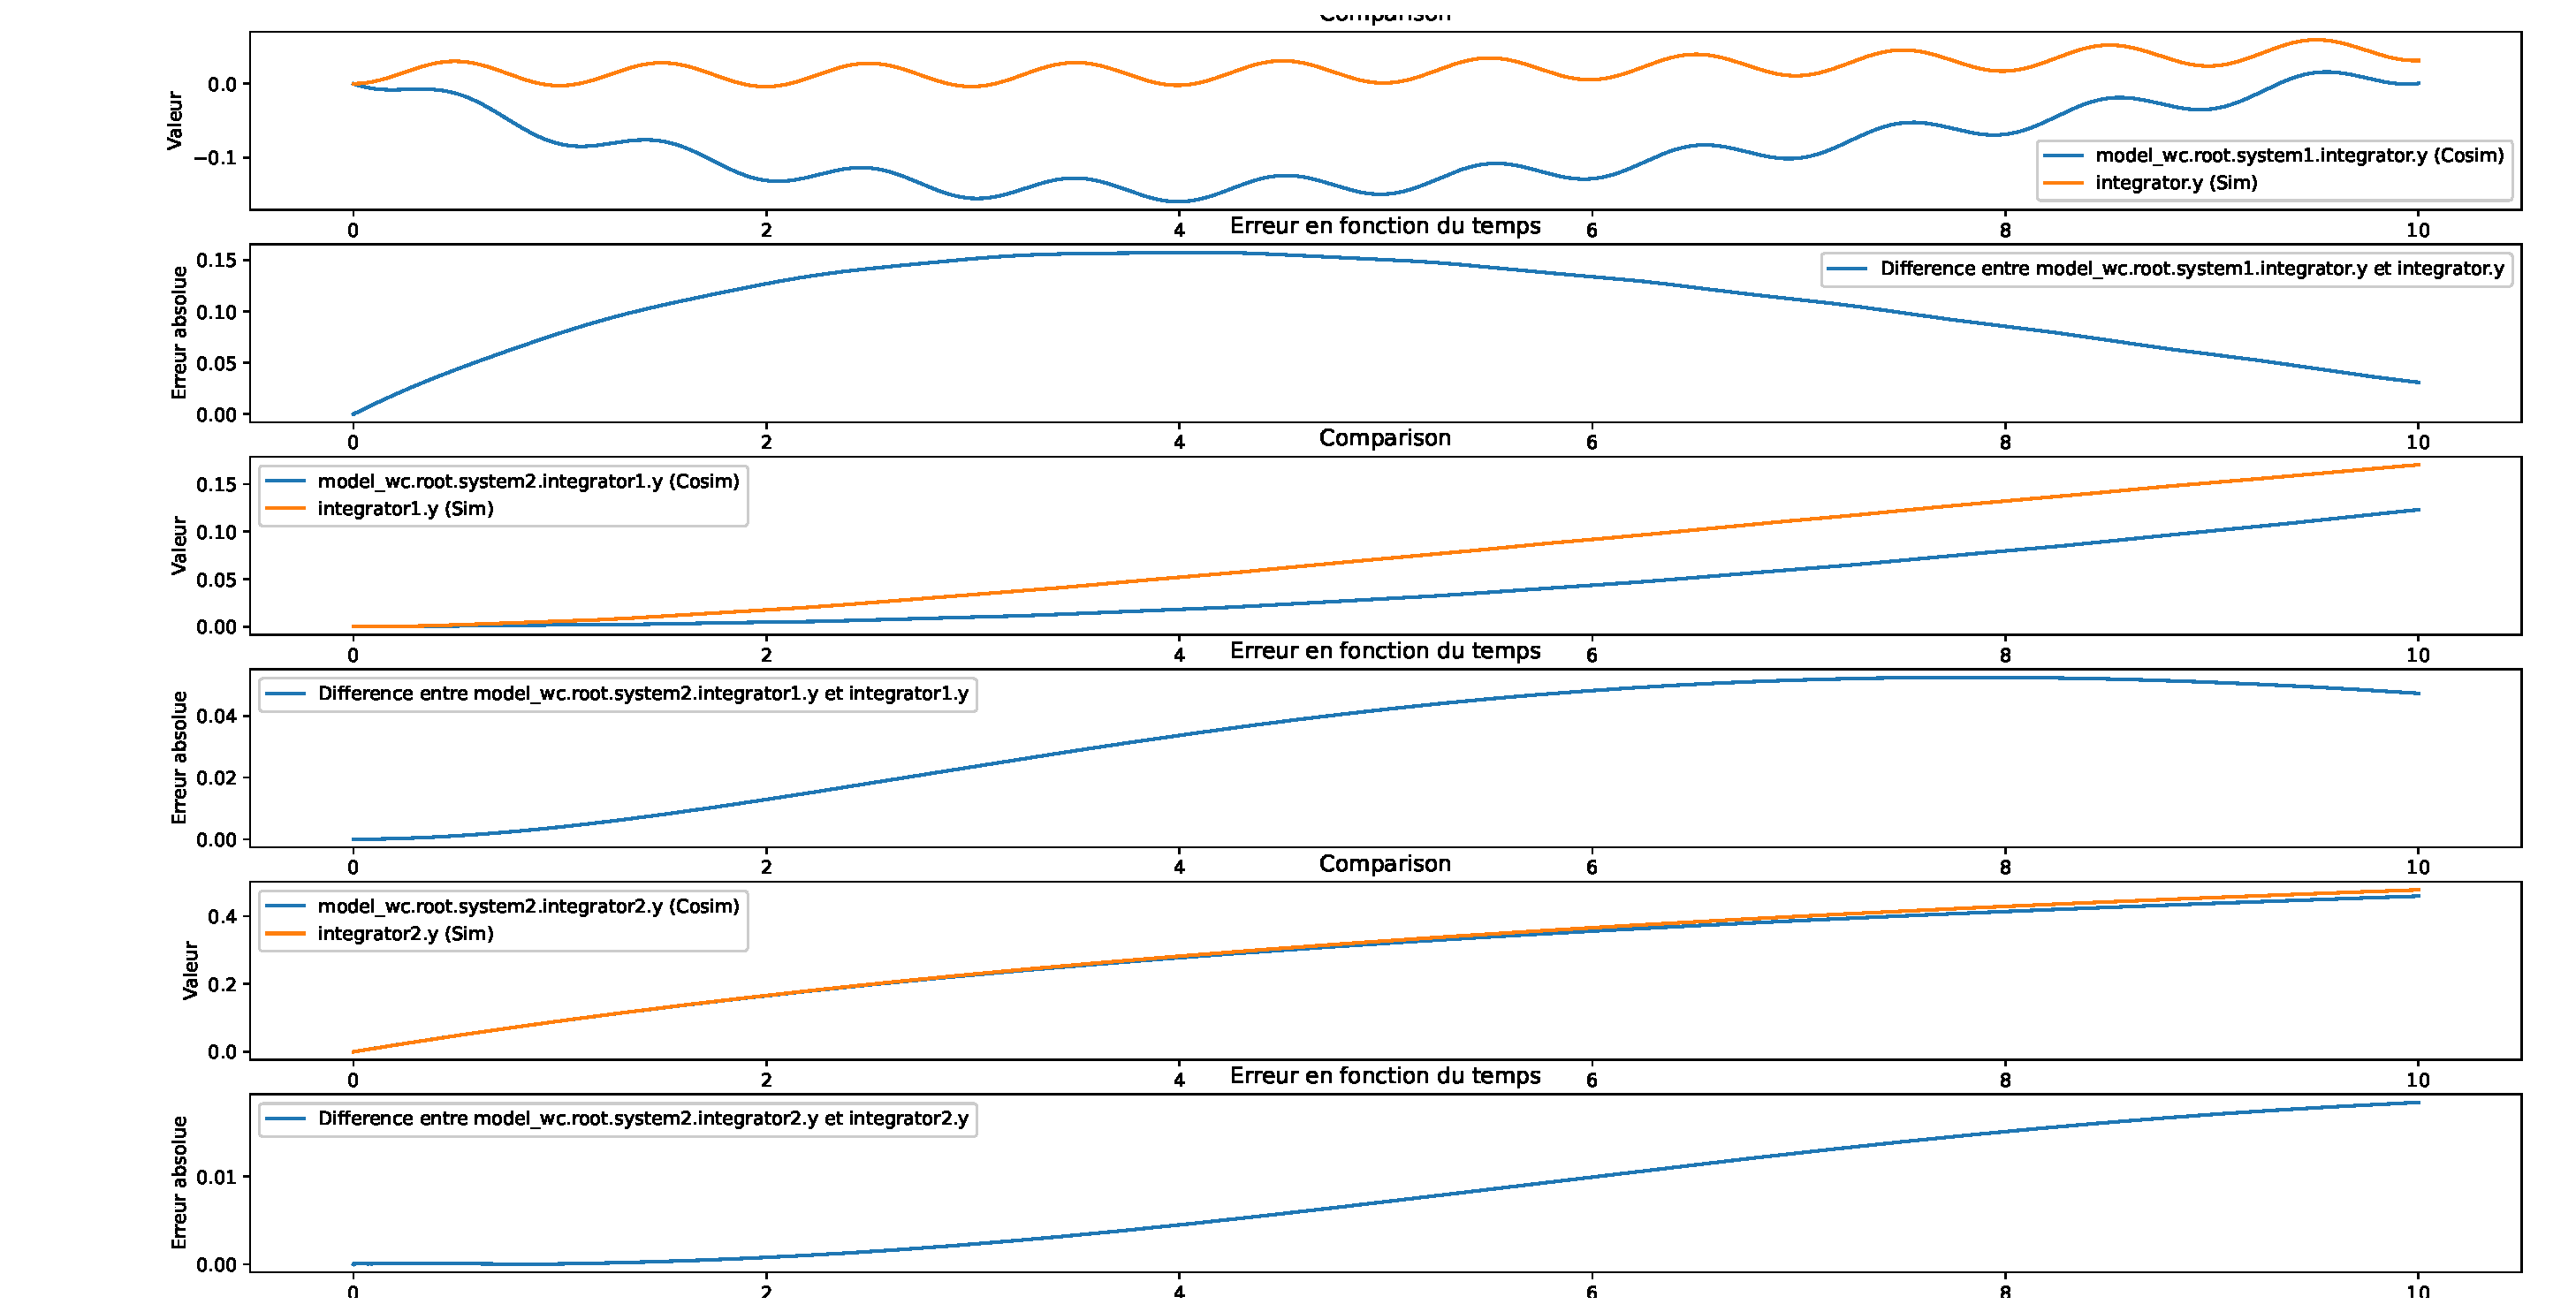
\includegraphics[width =\textwidth]{chainevolschwarz.eps}
    \caption{Comparaison de l'orchestrateur d'OMS avec une simulation monolithique du modèle \ref{fig:29}}
    \label{fig:28}
\end{figure}

\begin{figure}[hbt!]
    \centering
    \begin{minipage}[b]{0.4\textwidth}
        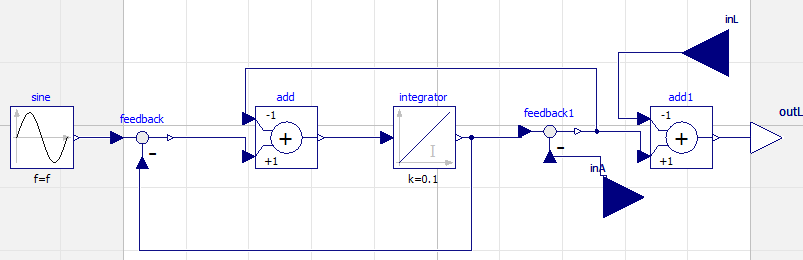
\includegraphics[width=\textwidth]{chainevolL.png}
    \end{minipage}
    \begin{minipage}[b]{0.4\textwidth}
      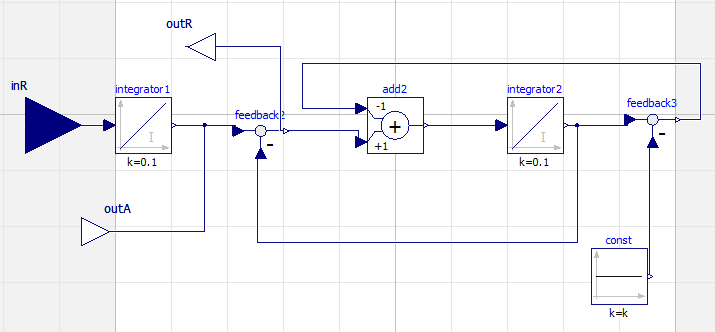
\includegraphics[width=\textwidth]{chainevolR.png}
  \end{minipage}
  \caption{Modèles utilisés dans la co-simulation d'une chaîne de contrôle de signal}
  \label{fig:29}
  \end{figure}
\newpage

La figure \ref{fig:29} représente une chaîne de traitement d'un signal, que l'on a découpée et exportée en FMUs, afin de comparer la simulation monolithique à la co-simulation avec la méthode d'Aitken-Schwarz dans \ref{fig:27} et l'orchestrateur à pas fixe d'OMS dans \ref{fig:28}.

\begin{figure}[hbt!]
    \centering
    \begin{minipage}[b]{0.45\textwidth}
        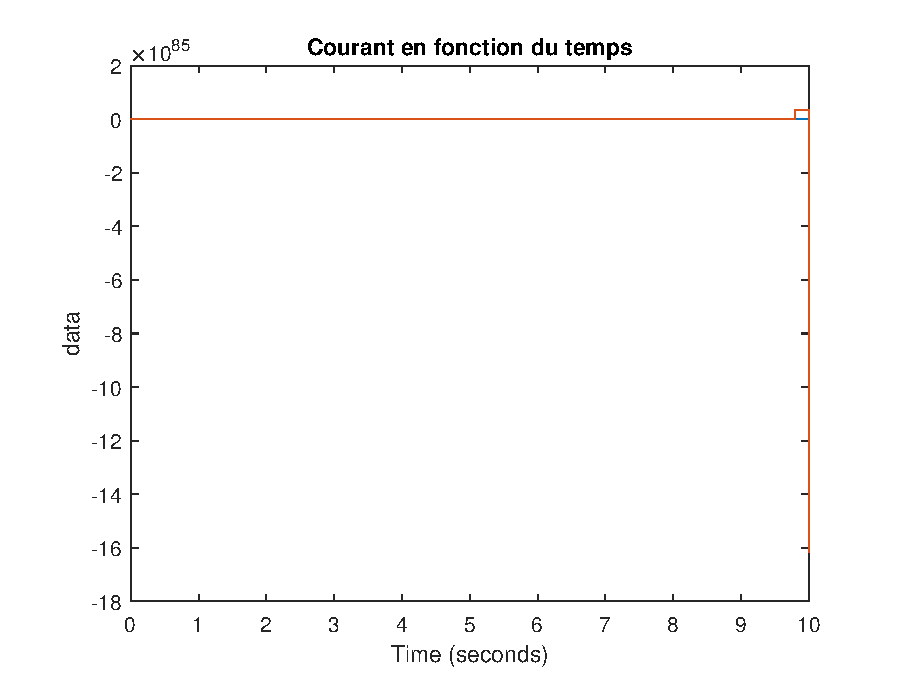
\includegraphics[width=\textwidth]{RL.eps}
        \caption{Résultats de la co-simulation du circuit RL sur Simulink}

    \end{minipage}
    \begin{minipage}[b]{0.45\textwidth}
      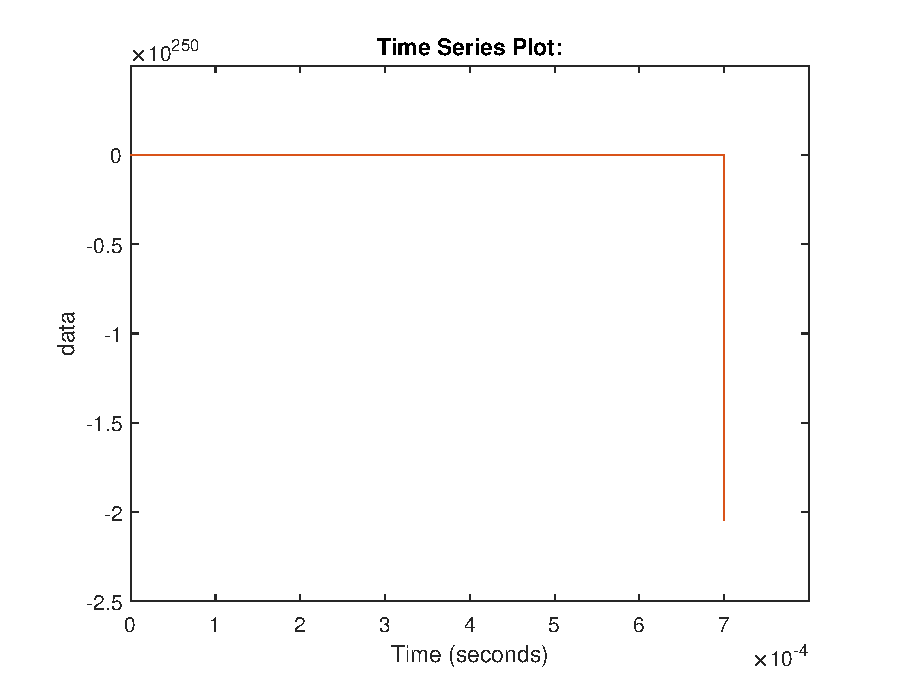
\includegraphics[width=\textwidth]{differenceAmplifier.eps}
      \caption{Résultats de la co-simulation de l'amplificateur différentiel \ref{fig:21} }
  \end{minipage}
  \label{fig:31}
  \end{figure}
  La figure \ref{fig:31} illustre les résultats obtenus via la co-simulation utilisant l'orchestrateur de SIMULINK. Cet orchestrateur appartient à la catégorie des algorithmes qui ne recourent pas à des fonctionnalités avancées telles que la capacité de faire un rollback, la modification des dérivées ou la sérialisation des données.

\section{Conclusion et perspectives}
En conclusion de ce chapitre, nous avons exploré les plateformes de co-simulation et les algorithmes d'orchestration, mettant en lumière leur importance cruciale dans la gestion efficace et précise des simulations complexes. À travers une analyse comparative des plateformes open source disponibles, nous avons identifié OMSimulator comme étant particulièrement adapté à nos besoins en raison de sa robustesse, sa documentation exhaustive, et sa capacité à intégrer diverses configurations de co-simulation. L'implémentation de l'algorithme d'orchestration Aitken-Schwarz a démontré des avantages significatifs en termes de gestion des erreurs et de la stabilité des simulations, confirmant ainsi l'efficacité de notre approche sélectionnée. Effectivement, on observe que l'erreur présentée dans la figure \ref{fig:24} atteint une magnitude de $0.14$, alors que dans la figure \ref{fig:25}, elle est réduite à $0.012$. Cette réduction montre que la méthode Aitken-Schwarz améliore les performances de la simulation par un facteur de 10 par rapport à la méthode par défaut d'OMS. Par ailleurs, dans la figure \ref{fig:26}, l'erreur est de $1.05\cdot 10^{-4}$. Cependant, la figure \ref{fig:31} révèle que la co-simulation a divergé, en raison de la présence d'une boucle algébrique (DAE), illustrant ainsi les avantages significatifs de la méthode Aitken-Schwarz. Pourtant, comme remarqué dans les figures \ref{fig:27}, \ref{fig:28}, les deux orchestrateurs ne parviennent pas à égaler les performances de la simulation monolithique. Cette limitation est attribuable au caractère très dynamique du système et à la manière dont il a été segmenté. En effet, le système comprend plusieurs intégrateurs, soulignant ainsi la nécessité d'adopter une méthode prédictive pour améliorer la précision de la co-simulation.